\section{System Overview}
\label{sec:systemoverview}



% Give an explanation and put the figure from steve's presentation on all of the components which should form the taxi scenario
% components in servicemix should comply the jbi specification, so the created service assemblies and deployed by the jbimulti2 should be jbi friendly. Furthermore they should be converted before deploying it with servicemix to base64
% main use case of the taxi scenario (with authentication, with the precondition of tenant is registered, etc etc and has deployed an http soap endpoint). Pick use cases from steffan's master thesis

%The taxi application is built up of different components running on 4 different servers with a Java 6 jdk. The JOnAS v 5.3.0 hosts the management and logic of the application. Each of the tenants deploy their TaxiCompany Web interface for taxi requestors' usage and the TaxiTransmitter for the taxi drivers' usage. Both of the interfaces have to be tenant aware in order to communicate through the tenant aware endpoints. As exposed before, a tenant's request is routed between two tenant aware endpoints if a successful tenant authentication occurs. The communication to and from the main BPEL processes (TaxiServiceProvider and ContextIntegration, see Figure \ref{fig:systemoverview}) is done through the \ac{ESB}. We must indicate that the BPEL processes are non multi-tenant aware and they receive and reply \ac{SOAP} over \ac{HTTP} requests and responses respectively. Hereby the \ac{ESB} must handle both tenant and non tenant aware routing between this components, as well as between the main BPEL processes, CMF, and GoogleServices adapters), by being able to create both tenant aware and non tenant aware endpoints.  

To provide transparent access support for migrated data, we present in this section an overview of the system, and its components. As we can see in Figure \ref{fig:systemoverview}, we divide the system into two main parts: the \term{Cloud Data Migration Application}, and the Cloud data access subsystem, which we name in this diploma thesis CDASMix (Cloud Data Access Support in ServiceMix-mt). However, in this diploma thesis we do not focus on the \term{Cloud Data Migration Application}, but include it in the system's overview in order to explain the role of CDASMix in the context of the migration of the DL to the Cloud. We consider the different tenant's applications hosted in their environment not as part of our system, but as consumers of the services provided by it. We must specify that the system overview described in Figures \ref{fig:systemoverview} and \ref{fig:componentoverview} shows the state after the data migration, when the data is already hosted in the backend Cloud provider. However, we include the migration process explanation in this section.

In the first part of our system, the \term{Cloud Data Migration Application} provides support for the data migration process, from an traditional to a Cloud data store, or between Cloud data stores \cite{bachmann2012}. After the tenant provides the required source and target data store configuration, the application calculates possible incompatibilities between data sources, and presents them to the tenant. If they exist, the tenant must resolve the incompatibilities before migrating the data. In the end phase of the migration process data can be easily migrated to the Cloud by providing the application with the \ac{DBMS} access credentials. 

From the point in time where the data migration process is terminated, either the application or the tenant must choose if he directly connects to his data source in the Cloud, or if he prefers to transparently access his data in the Cloud utilizing our Cloud-enabled data bus. If the latter is chosen, either the application or the tenant must register which communication protocol is required and register access and configuration data in our registry, e.g. database type, database URL, access credentials, etc. For this purpose, we enhance the administration and management system's (JBIMulti2) Web service \ac{API} with Cloud data access registering capabilities, as described in the following sections. 

\begin{figure}[htb]
	\centering
		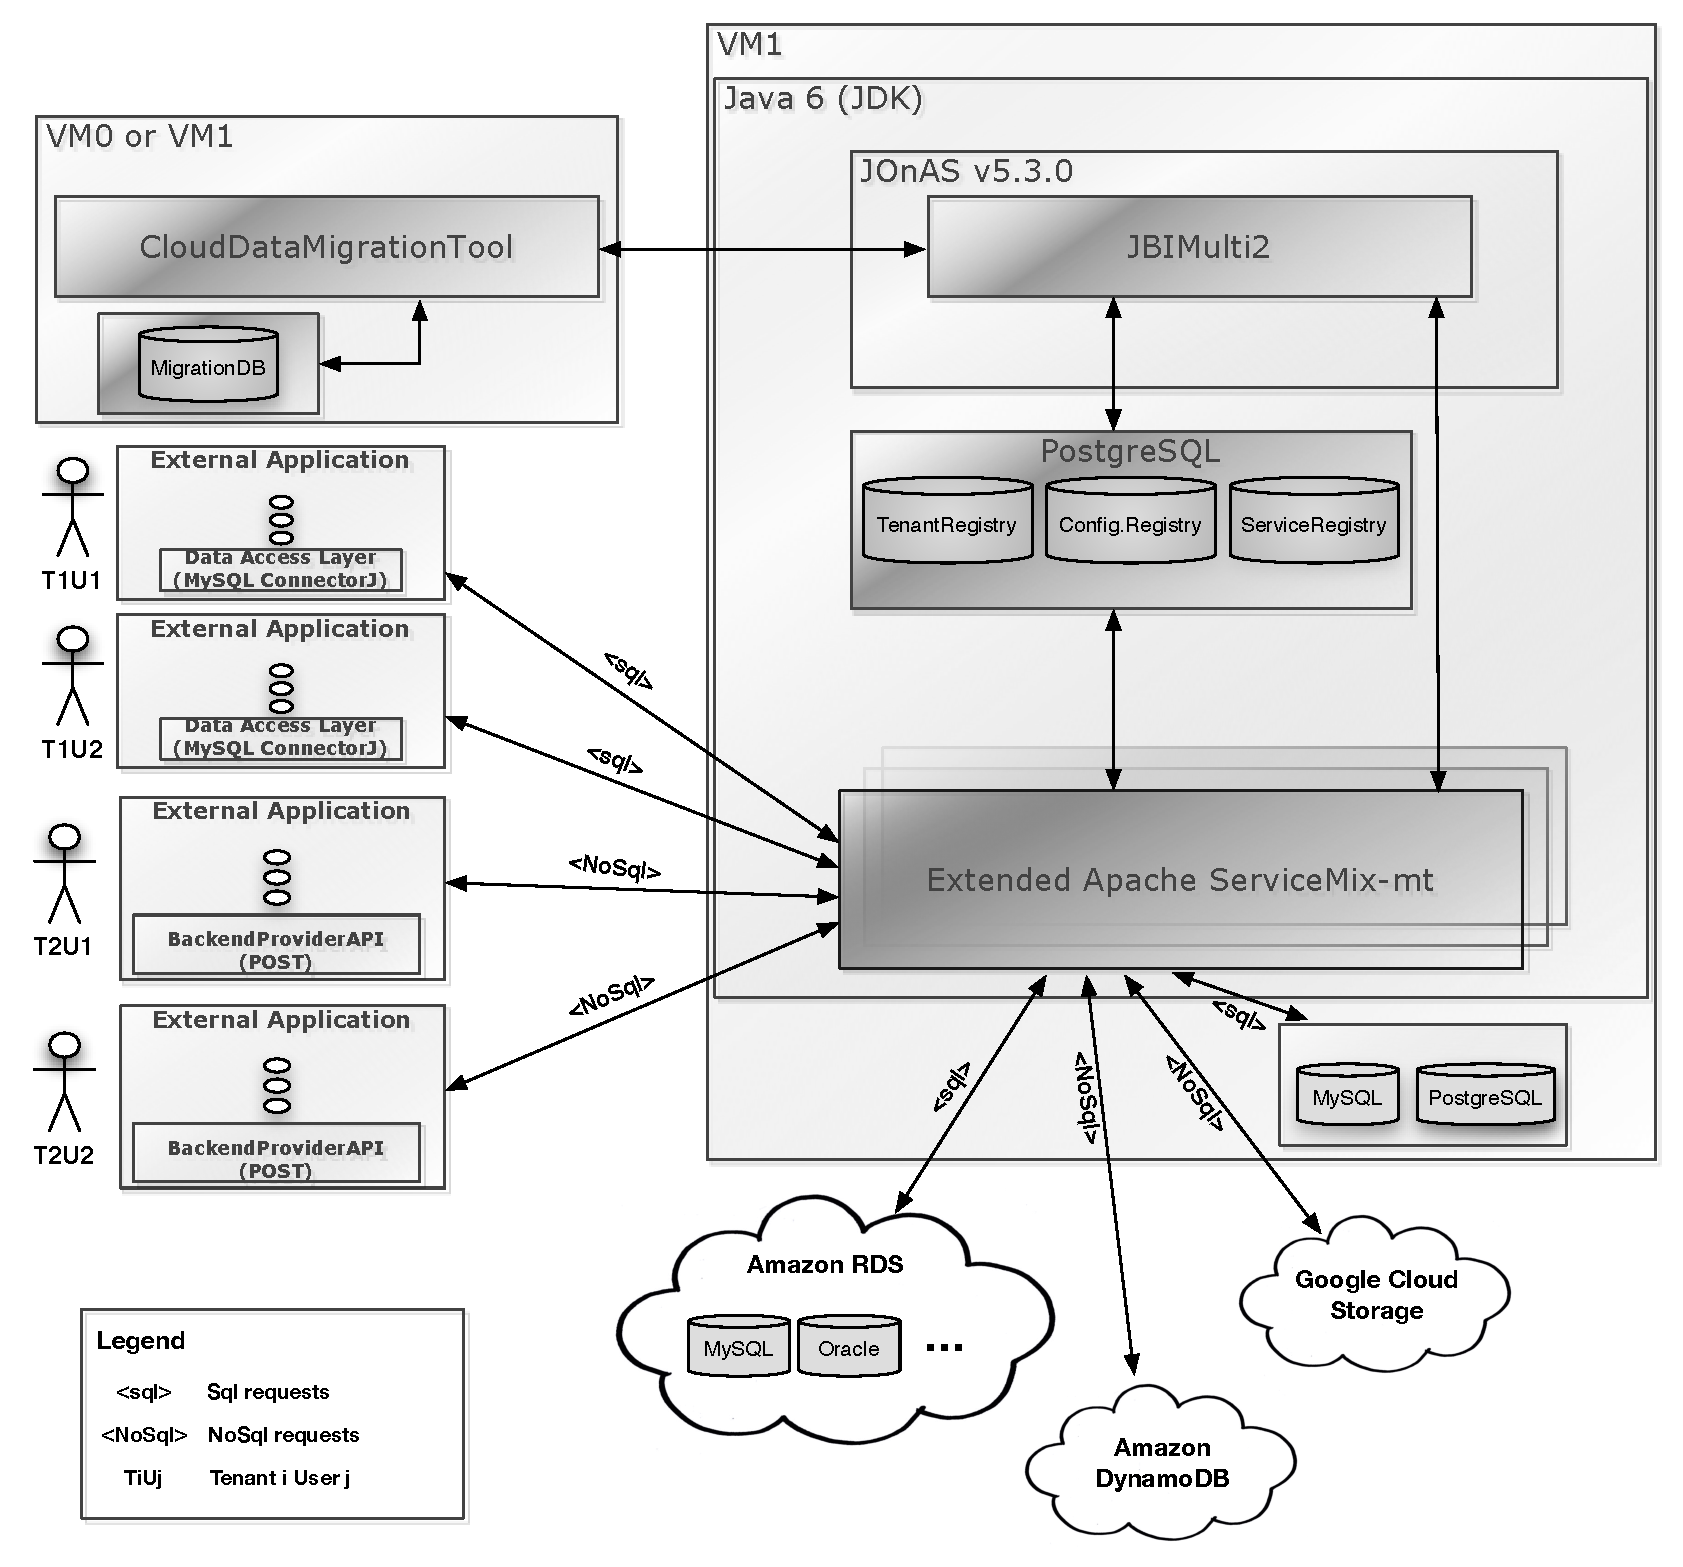
\includegraphics[clip, scale=0.5]{./gfx/systemoverview.pdf}
	\caption[Transparent Cloud Data Access System Overview]{Transparent Cloud data access system overview, including the \term{Cloud Data Migration Application} \cite{bachmann2012}. Note: represents the system in the post-migration phase}
	\label{fig:systemoverview}
\end{figure}

The transparent Cloud data access access support is achieved by the interaction of three main components: JBIMulti2, registries containing tenant-aware information, and an extended version of ServiceMix-mt (see Figure \ref{fig:systemoverview}). JBIMulti2 deploys in ServiceMix-mt the \ac{SA}s containing the endpoint and routing configurations selected by the tenant, which support two different communication protocols: MySQL and \ac{HTTP}. From this point the DAL of the tenant's application can retrieve and modify data in his data container in the Cloud through the \ac{ESB} connecting to a single logical endpoint which connects to multiple physical backend data stores. In our approach we provide also the possibility, either to configure a connection to the traditional database, e.g. when a hybrid model is pursued, or to utilize a \ac{DBMS} provided in our system, which is described in the following subsection.

%The JBIMulti2 utilizes three main components in the system: registries created in a PostgreSQL database, resources in ActiveMQ and ServiceMix. When deploying a tenant's \ac{SA} the application initiates an unidirectional communication to a management queue from which a management \ac{OSGi} bundle consumes the management messages from JBIMulti2 and performs managements operations in ServiceMix, such as deploy and undeploy. The deployed multi-tenant \ac{SA}s configure the tenants' endpoints for \ac{BC}s or \ac{SE}s. When deployed a multi-tenant \ac{SA} which packages a \ac{JMS} endpoint configuration, resources are transparently created in the out-of-the-box ActiveMQ instance which is shipped with ServiceMix. However, it is out of the scope of this student thesis an interface for connecting the different tenants with the created \ac{JMS} resources.


\FloatBarrier
\newpage